\documentclass{article}
\usepackage[utf8]{inputenc}
\usepackage[icelandic]{babel}
\usepackage[T1]{fontenc}
\usepackage{graphicx}
\usepackage{mathtools}
\usepackage{amsmath}
\usepackage{amssymb}
\usepackage{minted}


\graphicspath{ {./} }
\title{Verkleg æfing 6 - GHSR}
\author{ttb3@hi.is}
\date{\today}

\begin{document}
\maketitle

\section*{1.}
Verkefnið snérist um að útbúa ótaktvísan teljara sem telur frá 0 til 13

\section*{2.}
Ég byrjaði á að lesa mér til um JK-flip flops þar sem ég var ekki með þá alveg á hreinu. 
Þegar ég var kominn með ehv smá skilning á þeim dembdi ég mér í djúpu laugina og byrjaði að hanna rásina í LOGISIM. 
JK vippu hluti rásarinnar reyndist frekar einfaldur í uppsetningu og þá byrjaði ég á D vippu hlutanum. 
D vippu hlutinn var eitthvað sem ég hafði gert áður þannig hann tók enga stund. 
Mesti tíminn fór í að tengja output í rétta röð til að geta lesið út.

\section*{3.}
Verkefnið í heildina gekk frekar vel, það kom mér samt á óvart hversu langann tíma það tekur að fá síðustu töluna út.

\section*{4.}
Hérna er lokarásin í tveimur mismunandi stöðum. Ég prófaði að láta hana keyra alveg í gegn nokkrum sinnum og það gekk bara vel.
\begin{center}
    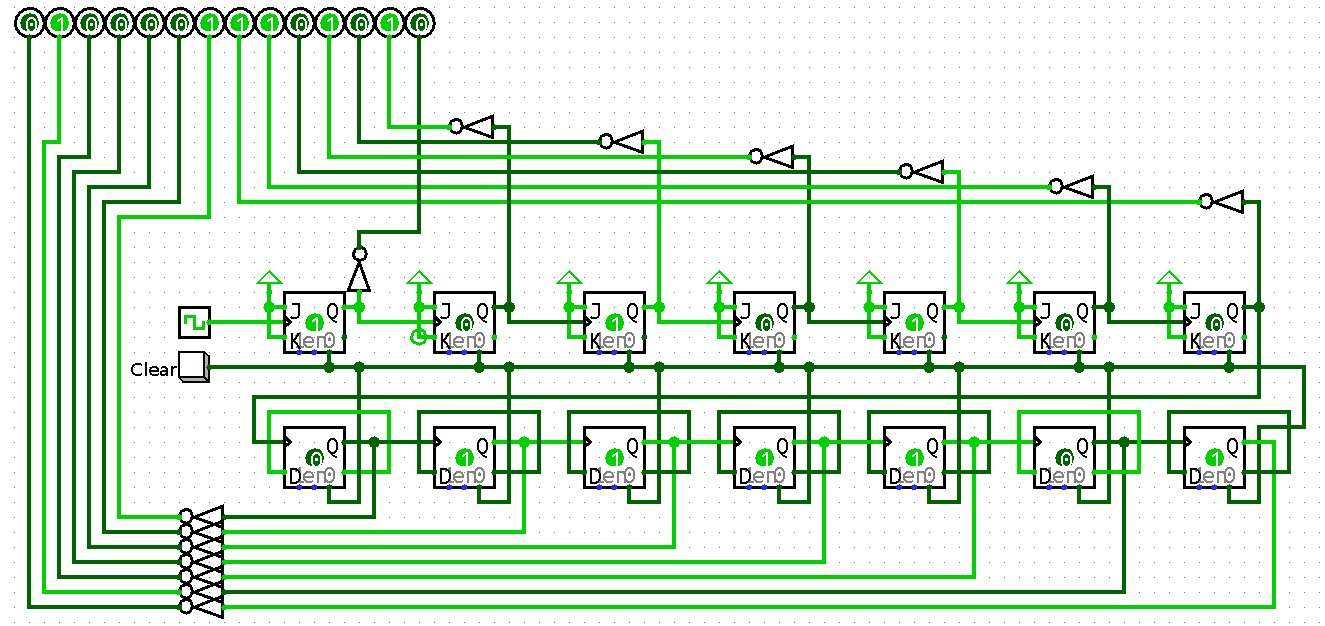
\includegraphics[scale=0.25]{Screenshot from 2022-04-09 13-01-42.png}
    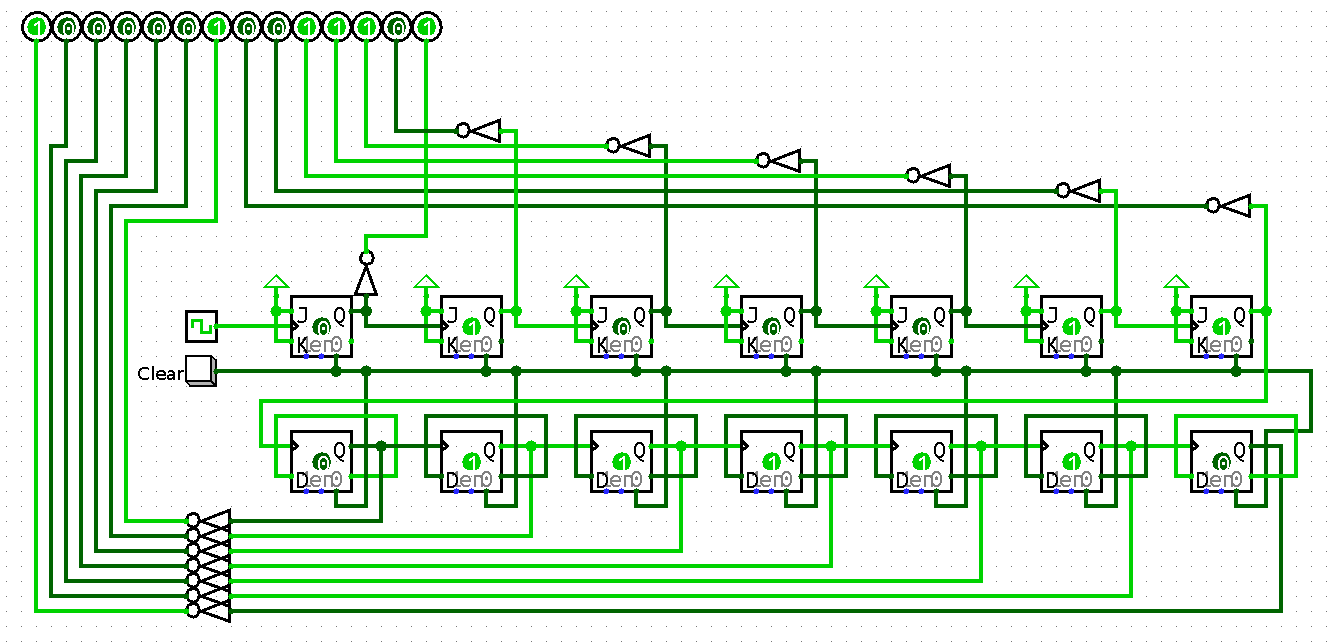
\includegraphics[scale=0.25]{Screenshot from 2022-04-09 13-03-20.png}
\end{center}

\end{document}